\documentclass{article}
\bibliographystyle{apacite} % Add the \bibliographystyle command to specify the bibliography style

% Useful packages
\usepackage[dutch]{babel} % Nederlands taalpakket
\usepackage{multicol}
\setlength{\columnsep}{1cm}
\setlength{\parskip}{1em}

% Set page size and margins
% Replace `letterpaper' with `a4paper' for UK/EU standard size
\usepackage[a4paper,top=2cm,bottom=2cm,left=2cm,right=2cm,marginparwidth=1.75cm]{geometry}

\usepackage{amsmath}
\usepackage{siunitx}
\usepackage{wrapfig}
\usepackage{float}
\usepackage{graphicx}
\graphicspath{{images/}}
\usepackage{subcaption}
\usepackage[colorlinks=true, allcolors=blue]{hyperref}
\usepackage{xcolor}
\usepackage{listings}
\usepackage{import}
\usepackage{xcolor}
\usepackage[toc,page]{appendix} % Pakket voor het maken van bijlagen
\usepackage{hyperref} % Pakket voor hyperlinks en verwijzingen
\usepackage{rotating}
\usepackage{array}
\usepackage{multirow}
\usepackage{lscape}
\usepackage{pdflscape}
\usepackage{longtable} % Add the longtable package to define the longtable environment
\usepackage{caption} % Add the caption package to use the \caption command
\usepackage{etex} % Add the etex package to use the \reserveinserts command
\usepackage{apacite} % APA citation style
\usepackage{booktabs}


% Definieer de kleuren voor syntax highlighting
\definecolor{codegreen}{rgb}{0,0.6,0}
\definecolor{codegray}{rgb}{0.5,0.5,0.5}
\definecolor{codepurple}{rgb}{0.58,0,0.82}
\definecolor{backcolour}{rgb}{0.95,0.95,0.92}



\lstdefinestyle{mystyle}{
    backgroundcolor=\color{backcolour},
    commentstyle=\color{codegreen},
    keywordstyle=\color{codepurple},
    numberstyle=\tiny\color{codegray},
    basicstyle=\footnotesize\ttfamily,
    breakatwhitespace=false,
    breaklines=true,
    captionpos=b,
    keepspaces=true,
    numbers=left,
    numbersep=5pt,
    showspaces=false,
    showstringspaces=false,
    showtabs=false,
    tabsize=2
}

\usepackage[dutch]{babel}% Language setting


\title{
    \begin{figure}[H]
        \centering
        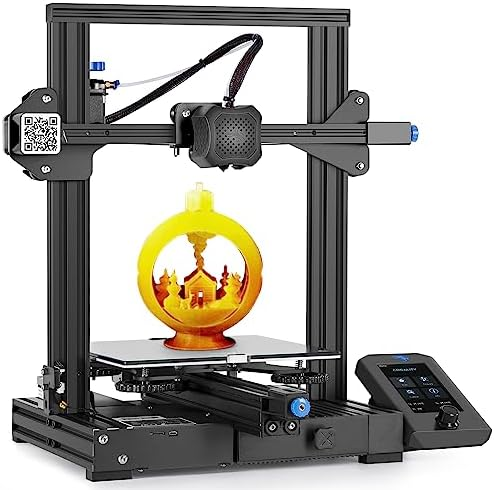
\includegraphics[scale = 1]{ender3.jpg} % Voeg hier de juiste afbeeldingsnaam in
    \end{figure}
    Life Cycle Engineering \\
    \large Uitvoeren van safety/reliability analyse}

\author{
  Vollmuller, Michel\\
  1809572\\
  \texttt{michel.vollmuller@student.hu.nl}
} 

\begin{document}
\maketitle

\tableofcontents

\setlength{\parindent}{0pt} % No indentation for new paragraphs

\newpage
\section{Opdracht}
\subsection{Inleiding}
In deze opdracht gaan we dieper in op het analyseren van technische objecten met als doel correctieve en preventieve maatregelen te identificeren om de prestaties te verbeteren en storingen te verminderen. Je zult verschillende technieken toepassen, zoals het opstellen van een functioneel schema, het uitvoeren van een FMEA/FTA (Fault Tree Analysis/Failure Mode and Effects Analysis), en het uitvoeren van een Pareto analyse.

\subsection{Doel}
Het doel van deze opdracht is om studenten vertrouwd te maken met diverse tools en methoden voor het analyseren van technische systemen, met de nadruk op het identificeren van oorzaken van storingen en het verbeteren van prestaties.

\subsection{Opdracht}
\begin{enumerate}
  \item Selectie van de opdracht
  \item Functioneel schema
  \item FMEA/FTA
  \item Pareto analyse
\end{enumerate}

Deze opdracht biedt studenten de mogelijkheid om praktijkervaring op te doen met het analyseren van technische systemen en het toepassen van troubleshooting technieken. Het bevordert ook het vermogen om gegevens te interpreteren, oorzaken te identificeren en oplossingen voor te stellen, wat essentiële vaardigheden zijn in diverse technische disciplines.

\subsection{scope}
Binnen dit verslag word er gekeken naar een Creality Ender 3 V2 3D-printer. De Creality Ender 3 V2 is een populaire 3D-printer die wordt gebruikt voor het maken van driedimensionale objecten door laag voor laag materiaal toe te voegen. Het systeem bestaat uit verschillende componenten die samenwerken om het printproces te voltooien. In dit verslag zullen we specifiek kijken naar het elektrische gedeelte van de printer. Hiervan zullen we een functioneel schema opstellen, een FMEA/FTA uitvoeren en een Pareto analyse maken.

\newpage

\section{Functioneel Schema}
\subsection{Inleiding}
Een functioneel schema is een schematische weergave van de werking van een technisch systeem. Een functioneel schema toont de verschillende componenten van het systeem en hun onderlinge relaties. Het doel van een functioneel schema is om een overzicht te geven van de werking van het systeem en de interactie tussen de verschillende componenten. Dit kan helpen bij het identificeren van storingen en het verbeteren van de prestaties van het systeem. In deze sectie zullen we een functioneel schema opstellen voor de Creality Ender 3 V2 3D-printer.

\subsection{Categorieën}
De Creality Ender 3 V2 3D-printer is een populaire 3D-printer die wordt gebruikt voor het maken van driedimensionale objecten door laag voor laag materiaal toe te voegen. Het systeem bestaat uit verschillende componenten die samenwerken om het printproces te voltooien. Binnen de context van een functioneel schema kunnen we de volgende categorieën onderscheiden:
\begin{itemize}
  \item Ingang
  \item Signal Processing
  \item Uitgang
  \item Voeding
  \item User interface
\end{itemize}

Binnen deze categorieën kunnen we de verschillende componenten van de 3D-printer identificeren en hun onderlinge relaties beschrijven. Dit zal ons helpen om een beter begrip te krijgen van de werking van de 3D-printer. De verschillende relaties zijn aangeduid met pijlen die de richting van de gegevensstroom aangeven. De pijlen zijn met kleurcodering aangegeven om de verschillende categorieën te onderscheiden.

\subsection{Onderdelen}
\textbf{Ingang}
\begin{itemize}
  \item End Switches\\
  Hiervan zitten er 2 op de Creality Ender 3 V2, een voor de X-as en een voor de Y-as. Deze worden gebruikt om de printer te kalibreren en de positie van de nozzle te bepalen.
  \item Bed Temperatuur\\
  Dit is een thermistor die de temperatuur van het heated bed meet. Dit is belangrijk voor het printproces, omdat de temperatuur van het bed van invloed is op de hechting van het filament. Wat directe invloed heeft op de kwaliteit van de print.
  \item Nozzle Temperatuur\\
  Dit is een thermistor die de temperatuur van de hotend meet. Dit is belangrijk voor het printproces, omdat de temperatuur van de hotend van invloed is op het smelten van het filament. Wat directe invloed heeft op de kwaliteit van de print.
  \item Probe\\
  Dit is een sensor die de hoogte van het bed meet. Dit is belangrijk voor het printproces, omdat de hoogte van het bed van invloed is op de hechting van het filament. De probe word voornamelijk gebruikt voor het automatisch levelen van het bed in het calibratie proces.
\end{itemize}

\textbf{Signal Processing}
\begin{itemize}
  \item Moeder Board\\
  Dit is het brein van de 3D-printer. Het moederbord ontvangt de signalen van de verschillende sensoren en stuurt de motoren en heaters aan. Het moederbord bevat ook de firmware die de printer aanstuurt.
\end{itemize}

\textbf{Uitgang}
\begin{itemize}
  \item Stepper motor X\\
  Dit is de motor die de X-as van de printer aanstuurt. De motor beweegt de nozzle horizontaal over het printbed.
  \item Stepper motor Y\\
  Dit is de motor die de Y-as van de printer aanstuurt. De motor beweegt het printbed horizontaal onder de nozzle.
  \item Stepper motor Z\\
  Dit is de motor die de Z-as van de printer aanstuurt. De motor beweegt het printbed verticaal omhoog en omlaag. Hiervan zijn er 2, een voor de linker en een voor de rechter kant van de arm waar X-as over beweegt.
  \item Heated Bed\\
  Dit is het verwarmde bed waarop het object wordt geprint. Het heated bed wordt verwarmd om de hechting van het filament te verbeteren.
  \item Hotend\\
  Dit is het verwarmde uiteinde van de printer waar het filament wordt gesmolten. Het hotend is verantwoordelijk voor het extruderen van het filament en het vormen van het object.
  \item Hotend Fan\\
  Dit is de ventilator die het geëxtrudeerde filament koelt zodat het snel hard word en niet meer kan vervormen.
\end{itemize}

\textbf{Voeding}
\begin{itemize}
  \item Power Supply\\
  De power supply converteert de netspanning naar de benodigde spanning voor de verschillende componenten van de printer.
\end{itemize}

\textbf{User interface}
\begin{itemize}
  \item Display\\
  Het display is het scherm waarop de gebruiker de printer kan bedienen en de status van het printproces kan volgen. Dit is de enigste plek waar de gebruiker interactie heeft met de printer.
\end{itemize}

\subsection{FMEA Schema}
\begin{figure}[H]
  \centering
  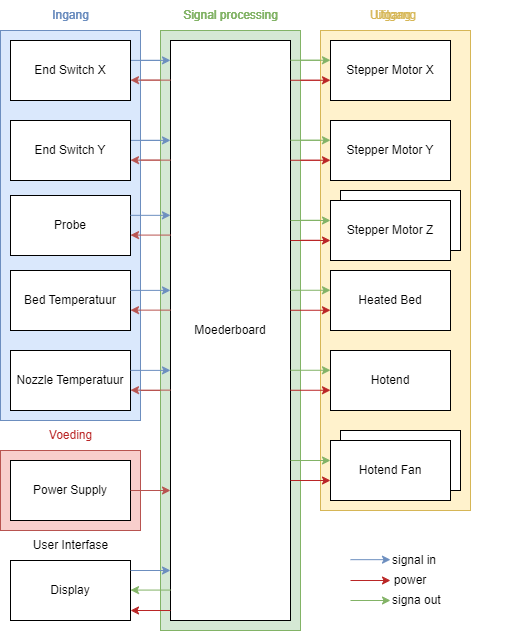
\includegraphics[width=\textwidth]{Creality Ender V2.drawio.png}
\end{figure}


\newpage

\section{FMEA}
\subsection{Inleiding}
Een FMEA (Failure Mode and Effects Analysis) is een systematische methode om potentiële storingen in een systeem te identificeren en te evalueren. Het doel van een FMEA is om de oorzaken van storingen te identificeren en de gevolgen van deze storingen te beoordelen. Dit kan helpen bij het nemen van preventieve stappen om storingen te voorkomen en de prestaties van het systeem te verbeteren. In deze sectie zullen we een FMEA uitvoeren voor de elektrische componenten van de Creality Ender 3 V2 3D-printer.

\subsection{Methode}
Bij het uitvoeren van een FMEA worden worden alle verschillende componenten van het systeem geanalyseerd en worden de mogelijke storingen geïdentificeerd en beoordeelt. Tijdens het onderzoek naar geschikte beoordelingstabellen kwam ik niet een tabel tegen wat voldoende aansluit bij dit onderwerp. Daarom heb ik zelf beoordelingstabellen gemaakt die hieronder te zien zijn.

\textbf{Severity:} De ernst van de storing, op een schaal van 1 tot 10, waarbij 1 de minst ernstige en 10 de meest ernstige is.
\begin{table}[!ht]
  \centering
  \begin{tabular}{|c|p{6.5cm}|p{6.5cm}|}
    \hline
    \textbf{Severity} & \textbf{Beschrijving} & \textbf{Veerbeeld in de 3D-printer Productie}\\ 
    \hline
      10 
    & Katastrofisch: Levensbedreigend of veiligheidskritisch; leidt tot productuitval die een gevaar voor gebruikers veroorzaakt. 
    & Kortsluiting in het elektrische systeem die brand veroorzaakt.\\
    \hline
    9&
    Zeer ernstig: Veroorzaakt ernstige productuitval; grote impact op de functionaliteit en veiligheid, maar geen direct gevaar voor het leven.&
    Motoren falen tijdens gebruik waardoor de printer oncontroleerbaar wordt.\\
    \hline
    8&
    Ernstig: Leidt tot aanzienlijke productuitval; product niet bruikbaar, grote reparaties nodig.&
    De extruder blokkeert volledig waardoor geen enkel printproces voltooid kan worden.\\
    \hline
    7&
    Hoog: Ernstige defecten; aanzienlijke vermindering van prestatie of functionaliteit, product moet worden gerepareerd.&
    Het verwarmingsbed bereikt niet de vereiste temperatuur, waardoor prints mislukken.\\
    \hline
    6&
    Matig-hoog: Vermindert prestatie aanzienlijk; product kan beperkt gebruikt worden of heeft frequente reparaties nodig.&
    Onbetrouwbare z-as beweging waardoor geprinte objecten scheef of misvormd raken.\\
    \hline
    5&
    Matig: Beïnvloedt prestatie en betrouwbaarheid; product functioneert, maar met beperkingen en verminderde efficiëntie.&
    Filament loopt regelmatig vast, wat handmatige interventie vereist om het printproces voort te zetten.\\
    \hline
    4&
    Matig-laag: Minder ernstige defecten; lichte vermindering van prestatie, maar het product blijft functioneel met minimale storingen.&
    Geluidsniveau van de printer is hoger dan verwacht, wat storend kan zijn in een stille omgeving.\\
    \hline
    3	&
    Laag: Kleine defecten die de gebruikservaring beïnvloeden, maar het product functioneert nog steeds binnen acceptabele normen.	&
    Kleine afwijkingen in de afmetingen van geprinte objecten, die niet kritisch zijn voor het eindgebruik.\\
    \hline
    2	&
    Zeer laag: Verwaarloosbare defecten; geen noemenswaardige invloed op prestatie of functionaliteit.	&
    Kleine cosmetische gebreken aan de behuizing van de printer.\\
    \hline
    1	&
    Verwaarloosbaar: Geen invloed op prestaties of functionaliteit; defecten zijn vrijwel onmerkbaar voor de gebruiker.&	
    Lichte krasjes of kleurverschillen op niet-zichtbare delen van de printer.\\
    \hline
  \end{tabular}
\caption{Severity Rating Scale}
\label{tab:Severity}
\end{table}

\textbf{Occurrence:} De waarschijnlijkheid dat de storing optreedt, op een schaal van 1 tot 10, waarbij 1 de minst waarschijnlijke en 10 de meest waarschijnlijke is.

\begin{table}[h!]
  \centering
  \begin{tabular}{|c|p{6.5cm}|p{6.5cm}|}
    \hline
    \textbf{Occurrence} & \textbf{Beschrijving} & \textbf{Frequentie}\\ 
    \hline
      10 
    & Zeer hoog: Bijna zeker dat de fout optreedt; komt regelmatig voor.	&
    minder dan 1 keer per dag\\
    \hline
    9&
    Zeer hoog: Verwacht vaak voor te komen; storingen zijn zeer waarschijnlijk.	&
    1 keer per dag\\
    \hline
    8&
    Hoog: Komt vaak voor; storingen zijn frequent.	&
    1 keer per week\\
    \hline
    7&
    Hoog: Komt regelmatig voor; storingen komen vaak voor.	&
    1 keer per maand\\
    \hline
    6&
    Matig hoog: Komt af en toe voor; storingen zijn niet ongewoon.	&
    1 keer per 3 maanden\\
    \hline
    5&
    Matig: Komt soms voor; storingen zijn occasioneel.	&
    1 keer per 6 maanden\\
    \hline
    4&
    Matig laag: Komt zelden voor; storingen zijn ongebruikelijk.	&
    1 keer per jaar\\
    \hline
    3	&
    Laag: Komt zeer zelden voor; storingen zijn zeer ongewoon.	&
    1 keer per 3 jaar\\
    \hline
    2	&
    Zeer laag: Bijna nooit voorkomend; storingen zijn uitzonderlijk.	&
    1 keer per 5 jaar\\
    \hline
    1	&
    Uitzonderlijk: Bijna onmogelijk dat de fout optreedt; storingen zijn extreem zeldzaam.	&
    meer dan 1 keer per 5 jaar\\
    \hline
  \end{tabular}
\caption{Occurance Rating Scale}
\label{tab:Occurance}
\end{table}

\newpage
\textbf{Detection:} De waarschijnlijkheid dat de storing wordt gedetecteerd voordat deze optreedt, op een schaal van 1 tot 10, waarbij 1 de minst waarschijnlijke en 10 de meest waarschijnlijke is.

\begin{table}[h!]
  \centering
  \begin{tabular}{|c|p{6.5cm}|p{6.5cm}|}
    \hline
    \textbf{Detection} & \textbf{Beschrijving} & \textbf{Frequentie}\\ 
    \hline
      10 
    & Zeer onwaarschijnlijk: De fout wordt bijna zeker niet gedetecteerd voor deze tot een storing leidt.	&
    Geen controles of detectiemogelijkheden beschikbaar.\\
    \hline
    9&
    Zeer laag: Zeer lage kans dat de fout wordt gedetecteerd voor deze tot een storing leidt.	&
    Zeer beperkte controles; slechts zelden effectief.\\
    \hline
    8&
    Laag: Lage kans dat de fout wordt gedetecteerd voor deze tot een storing leidt.	&
    Weinig effectieve controles; fouten worden meestal niet gedetecteerd.\\
    \hline
    7&
    Laag: Matige kans dat de fout wordt gedetecteerd voor deze tot een storing leidt.	&
    Enkele controles aanwezig, maar vaak niet effectief.\\
    \hline
    6&
    Matig: Redelijke kans dat de fout wordt gedetecteerd voor deze tot een storing leidt.	&
    Standaard controles aanwezig, maar niet altijd betrouwbaar.\\
    \hline
    5&
    Matig: Gelijkmatige kans dat de fout wordt gedetecteerd voor deze tot een storing leidt.	&
    Standaard controles aanwezig en redelijk betrouwbaar.\\
    \hline
    4&
    Matig hoog: Hogere kans dat de fout wordt gedetecteerd voor deze tot een storing leidt.	&
    Effectieve controles aanwezig en vaak betrouwbaar.\\
    \hline
    3	&
    Hoog: Grote kans dat de fout wordt gedetecteerd voor deze tot een storing leidt.	&
    Zeer effectieve controles aanwezig, vaak betrouwbaar.\\
    \hline
    2	&
    Zeer hoog: Zeer grote kans dat de fout wordt gedetecteerd voor deze tot een storing leidt.	&
    Bijna volledige detectiemogelijkheden; fouten worden meestal gedetecteerd.\\
    \hline
    1	&
    Uitzonderlijk hoog: Bijna zekerheid dat de fout wordt gedetecteerd voor deze tot een storing leidt.	&
    Zeer betrouwbare en effectieve controles; fouten worden vrijwel altijd gedetecteerd.\\
    \hline
  \end{tabular}
\caption{Detection Rating Scale}
\label{tab:Detection}
\end{table}


\newpage
\begin{landscape}
    \subsection{FMEA Table}  \label{sec:FMEA Table} 
    \begin{longtable}{|l|l|l|c|c|c|c|l|}
        \hline
        \textbf{Item/Functie} & \textbf{Failure mode} & \textbf{Effect} & \textbf{Severity} & \textbf{Occurrence} & \textbf{Detection} & \textbf{RPN} & \textbf{Corr. Action} \\ \hline
        \multirow{3}{*}{Power Supply}       & Defect            & Geen voeding  & 4 & 3 & 2 & 24 & \\
                                            & Kortsluiting      & Geen voeding  & 6 & 3 & 5 & 90 & ader paren beter scheiden tegen kortsluiting\\
                                            & Onderbreking      & Geen voeding  & 4 & 2 & 2 & 16 & \\
                                            \hline
        \multirow{4}{*}{End Switch X}       & Sensor defect     & X Switch low  & 3 & 1 & 6 & 18 & \\
                                            & Geen voeding      & X Switch low  & 3 & 3 & 6 & 54 &  gerelateerd aan power supply\\
                                            & false true        & X Switch high & 2 & 1 & 7 & 14 & \\
                                            & false false       & X Switch low  & 2 & 1 & 7 & 14 & \\ 
                                            \hline
        \multirow{4}{*}{End Switch Y}       & Sensor defect     & Y Switch low  & 3 & 1 & 6 & 18 & \\
                                            & Geen voeding      & Y Switch low  & 3 & 3 & 6 & 54 & \\
                                            & false true        & Y Switch high & 2 & 1 & 7 & 14 & \\
                                            & false false       & Y Switch low  & 2 & 1 & 7 & 14 & \\ 
                                            \hline
        \multirow{4}{*}{Probe}              & Sensor defect     & Probe low  & 3 & 2 & 6 & 36 & \\
                                            & Geen voeding      & Probe low  & 3 & 3 & 6 & 54 & gerelateerd aan power supply\\
                                            & false true        & Probe high & 2 & 1 & 7 & 14 & \\
                                            & false false       & Probe low  & 2 & 1 & 7 & 14 & \\ 
                                            \hline
        \multirow{4}{*}{Bed Temperatuur}    & Sensor defect     & Bed Temperatuur low  & 3 & 1 & 6 & 18 & \\
                                            & Geen voeding      & Bed Temperatuur low  & 3 & 3 & 6 & 54 & gerelateerd aan power supply\\
                                            & false true        & Bed Temperatuur high & 2 & 1 & 7 & 14 & \\
                                            & false false       & Bed Temperatuur low  & 2 & 1 & 7 & 14 & \\ 
                                            \hline
        \multirow{4}{*}{Nozzle Temperatuur} & Sensor defect     & Nozzle Temperatuur low  & 3 & 1 & 6 & 18 & \\
                                            & Geen voeding      & Nozzle Temperatuur low  & 3 & 3 & 6 & 54 & gerelateerd aan power supply\\
                                            & false true        & Nozzle Temperatuur high & 2 & 1 & 7 & 14 & \\
                                            & false false       & Nozzle Temperatuur low  & 2 & 1 & 7 & 14 & \\ 
                                            \hline          
        \multirow{3}{*}{Display}            & Defect            & Geen display  & 4 & 2 & 3 & 24 & \\ 
                                            & Kortsluiting      & Geen display  & 6 & 1 & 4 & 24 & \\
                                            & Onderbreking      & Geen display  & 4 & 1 & 3 & 12 & \\
                                            \hline 
        \newpage
        \hline
        \textbf{Item/Functie} & \textbf{Failure mode} & \textbf{Effect} & \textbf{Severity} & \textbf{Occurrence} & \textbf{Detection} & \textbf{RPN} & \textbf{Corr. Action} \\ \hline
        \multirow{15}{*}{Moeder Board}      & Defect                    & printer werkt niet        & 9 & 1 & 2 & 18 & \\
                                            & Geen voeding              & printer werkt niet        & 9 & 3 & 3 & 81 & gerelateerd aan power supply\\
                                            & X Switch low              & X Stepper rotating        & 3 & 1 & 6 & 18 & \\
                                            & X Switch high             & X Stepper stop signal     & 5 & 1 & 4 & 20 & \\
                                            & Y Switch low              & Y stepper rotating        & 3 & 1 & 6 & 18 & \\
                                            & Y Switch high             & Y stepper stop signal     & 5 & 1 & 4 & 20 & \\
                                            & Probe low                 & Z Stepper rotating        & 3 & 1 & 6 & 18 & \\
                                            & Probe high                & Z Stepper stop signal     & 5 & 1 & 4 & 20 & \\
                                            & Bed Temperatuur low       & Heated Bed heating        & 4 & 1 & 6 & 24 & \\
                                            & Bed Temperatuur high      & Heated Bed not heating    & 5 & 1 & 5 & 25 & \\
                                            & \multirow{2}{*}{Nozzle Temperatuur low}    & Hotend heating            & 4 & 1 & 6 & 24 & \\
                                            &                                            & Hotend Fan standing stil  & 3 & 1 & 3 & 9 & \\
                                            & \multirow{2}{*}{Nozzle Temperatuur high}   & Hotend not heating        & 5 & 1 & 5 & 25 & \\
                                            &                                            & Hotend Fan rotating       & 4 & 1 & 6 & 24 & \\
                                            \hline
        \multirow{4}{*}{Stepper motor X}    & Defect                & Stepper motor not running             & 8 & 1 & 2 & 16 & \\
                                            & No power              & Stepper motor not running             & 8 & 1 & 2 & 16 & \\
                                            & X Stepper rotating    & Stepper motor overheating /burning    & 10 & 1 & 1 & 10 & \\
                                            & X Stepper stop signal & Stepper motor not running             & 8 & 1 & 2 & 16 & \\ 
                                            \hline 
        \multirow{4}{*}{Stepper motor Y}    & Defect                & Stepper motor not running             & 8 & 1 & 2 & 16 & \\
                                            & No power              & Stepper motor not running             & 8 & 1 & 2 & 16 & \\
                                            & Y Stepper rotating    & Stepper motor overheating /burning    & 10 & 1 & 1 & 10 & \\
                                            & Y Stepper stop signal & Stepper motor not running             & 8 & 1 & 2 & 16 & \\ 
                                            \hline
        \multirow{4}{*}{Stepper motor Z}    & Defect                & Stepper motor not running             & 8 & 1 & 2 & 16 & \\
                                            & No power              & Stepper motor not running             & 8 & 1 & 2 & 16 & \\
                                            & Z Stepper rotating    & Stepper motor overheating /burning    & 10 & 1 & 1 & 10 & \\
                                            & Z Stepper stop signal & Stepper motor not running             & 8 & 1 & 2 & 16 & \\ 
                                            \hline 
        \multirow{4}{*}{Heated Bed}         & Defect                    & Bed stays cool, Print wil not stick to the bed    & 4 & 1 & 3 & 12 & \\
                                            & No power                  & Bed stays cool, Print wil not stick to the bed    & 4 & 3 & 3 & 18 & \\
                                            & Heated bed heating        & Heated bed continuously heating, fire             & 10 & 1 & 2 & 20 & \\
                                            & Heated bed not heating    & Bed stays cool, Print wil not stick to the bed    & 2 & 2 & 3 & 12 & \\ 
                                            \hline 
        \multirow{4}{*}{Hotend}             & Defect                    & Hotend stays cool, Filament wil not melt          & 5 & 1 & 3 & 15 & \\
                                            & No power                  & Hotend stays cool, Filament wil not melt          & 7 & 3 & 3 & 63 & gerelateerd aan power supply\\
                                            & Hotend heating            & Hotend continuously heating, fire                 & 10 & 3 & 2 & 60 & overheat protection\\
                                            & Hotend not heating        & Hotend stays cool, Filament wil not melt          & 5 & 2 & 2 & 20 & \\ 
                                            \hline
        \multirow{4}{*}{Hotend Fan}         & Defect                    & Hotend Fan not rotating                           & 6 & 3 & 3 & 54 & overheat protection\\
                                            & No power                  & Hotend Fan not rotating                           & 7 & 3 & 3 & 63 & gerelateerd aan power supply\\
                                            & Hotend Fan rotating       & Hotend Fan continuously rotating                  & 6 & 4 & 1 & 24 & \\
                                            & Hotend Fan standing stil  & Hotend Fan not rotating                           & 7 & 4 & 2 & 56 & overheat protection\\ 
                                            \hline   
    \end{longtable}
    % \caption{FMEA Tabel Crrality Ender 3 V2 3D-printer}
    % \label{tab:FMEA Tabel}
\end{landscape}

\newpage

\subsection{Onderdelen}
In hoofdstuk \ref{sec:FMEA Table} is een FMEA tabel opgesteld voor de Creality Ender 3 V2 3D-printer. Hierin zijn de verschillende componenten van de printer geanalyseerd en zijn de mogelijke storingen geïdentificeerd en beoordeeld. De FMEA tabel geeft een overzicht van de verschillende storingen die kunnen optreden en de ernst, waarschijnlijkheid en detecteerbaarheid van deze storingen. Op basis van deze informatie kunnen we de risico's van de verschillende storingen beoordelen en corrigerende maatregelen nemen om de prestaties van de printer te verbeteren en storingen te voorkomen. In dit hoofdstuk gaan we dieper in op een aantal componenten van de printer en de mogelijke storingen die daarbij kunnen optreden.

\textbf{Voeding}

Een falende voeding kan ernstige gevolgen hebben voor de werking van de Ender 3 V2. Een defecte voeding kan leiden tot onverwachte uitschakelingen, wat kan resulteren in mislukte prints en mogelijke schade aan de printer (\citeNP{reddit_warning_2023}). Het probleem kan variëren van volledig verlies van stroom tot intermitterende stroomuitval, wat moeilijk te diagnosticeren en te repareren kan zijn.

Hoewel het moeilijk is om exacte statistieken te verkrijgen, zijn er meerdere meldingen van voedingstoringen bij de Ender 3 V2. Gebruikers op verschillende forums en online gemeenschappen hebben vergelijkbare problemen gerapporteerd (\citeNP{reddit_issues_2023}; \citeNP{stackexchange_random_2023}). Deze problemen lijken niet uitzonderlijk, wat suggereert dat de faalkans significant genoeg is om aandacht te verdienen. Wat vaak voorkomt is dat de voeding oververhit raakt en daardoor uitvalt of kortsluiting maakt. 

Het detecteren van een falende voeding is meestal vrij eenvoudig. Symptomen zijn onder andere de printer die niet aan gaat, of onverwacht uitschakelt tijdens gebruik (\citeNP{3dprintberry_power_2023}). Gebruikers kunnen vaak de oorzaak bevestigen door de voeding te controleren op visuele schade of door de spanning te meten met een multimeter. In veel gevallen is vervanging van de PSU de beste oplossing.

\textbf{CR Touch (Probe)}

Een falende CR Touch Sensor kan grote problemen veroorzaken tijdens het printproces. Fouten in de bed leveling kunnen leiden tot slechte hechting van de eerste laag, wat resulteert in mislukte prints en verspilling van materiaal (\citeNP{crealitycloud_2023}). In sommige gevallen kan een defecte sensor ervoor zorgen dat de printer helemaal niet meer functioneert, wat de noodzaak van een goed werkende sensor benadrukt.

Er zijn meerdere meldingen van problemen met de CR Touch Sensor op verschillende online platforms. Gebruikers rapporteren dat de sensor soms niet werkt of dat deze onregelmatig presteert (\citeNP{reddit_s0r9x1_2023}; \citeNP{github_mriscoc_2023}). Deze problemen lijken vaker voor te komen bij aftermarket producten zoals de CR Touch Sensor, wat suggereert dat de faalkans hoger is dan bij ingebouwde sensoren. Vaak komt dit door onjuiste installatie of kalibratie van de sensor.

Het detecteren van problemen met de CR Touch Sensor is relatief eenvoudig. Gebruikers merken vaak dat de sensor faalt tijdens het homing proces of dat er inconsistenties zijn tijdens het bed leveling (\citeNP{reddit_11anrgx_2023}; \citeNP{octoprint_2023}). Visuele inspectie en testcommando's kunnen helpen om de oorzaak van het probleem te identificeren. In sommige gevallen kunnen firmware-updates of herkalibratie de problemen oplossen, maar soms is vervanging van de sensor noodzakelijk (\citeNP{bigtreetech_2023}).

\textbf{Hotend}

Een falende hotend kan grote gevolgen hebben voor de printkwaliteit en veiligheid. Problemen zoals lage temperatuurfouten en thermische failures kunnen optreden, wat leidt tot mislukte prints en mogelijke schade aan de printer (\citeNP{reddit_low_temp_2023}; \citeNP{all3dp_thermal_2023}). Thermische failures zijn bijzonder gevaarlijk omdat ze kunnen leiden tot oververhitting en zelfs brandgevaar (\citeNP{reddit_fire_hazard_2023}).

Er zijn meerdere meldingen van hotend problemen bij de Ender 3 V2. Veel gebruikers hebben problemen gerapporteerd met het handhaven van de juiste temperatuur, wat vaak resulteert in foutmeldingen en oververhitte hotend want brandgevaar oplevert (\citeNP{crealitycloud_heating_failed_2023}; \citeNP{reddit_mk8_2023}). Deze problemen komen regelmatig voor, wat suggereert dat de faalkans significant is en dat gebruikers zich bewust moeten zijn van mogelijke problemen.

Het detecteren van problemen met de hotend is meestal eenvoudig. Symptomen zijn onder andere foutmeldingen zoals "Heating Failed" of "Low Temperature Error" (\citeNP{reddit_low_temp_2023}; \citeNP{crealitycloud_heating_failed_2023}). Visuele inspectie van de hotend kan ook tekenen van schade of slijtage onthullen. Daarnaast kunnen gebruikers temperatuurmetingen uitvoeren met een infraroodthermometer om de prestaties van de hotend te controleren.

\textbf{Cooling fan}

Een falende cooling fan kan leiden tot oververhitting van de nozzle en slechte koeling van het geprinte object, wat resulteert in mislukte prints en mogelijke schade aan de hotend (\citeNP{stackexchange_2023}; \citeNP{reddit_q2etpz_2023}). Zonder adequate koeling kunnen onderdelen van de printer oververhit raken, wat kan leiden tot versnelde slijtage of zelfs brandgevaar (\citeNP{reddit_hvscjl_2023}).

Er zijn verschillende meldingen van problemen met de cooling fan bij de Ender 3 V2. Gebruikers hebben gerapporteerd dat zowel de nozzle fan als de part cooling fan soms niet werken, dit kan resulteren in een hotend waarbij de temperatuur niet goed geregeld kan worden wat in ergste gevallen risico op brand kan opleveren (\citeNP{stackexchange_2023}; \citeNP{reddit_q2etpz_2023}; \citeNP{3dprintboard_2023}). Deze problemen lijken regelmatig voor te komen, wat suggereert dat de faalkans significant is en dat gebruikers zich bewust moeten zijn van mogelijke problemen.
 
Het detecteren van problemen met de cooling fan is meestal eenvoudig. Symptomen zijn onder andere een merkbare afname in koelprestaties, ongewone geluiden of volledige uitval van de fan (\citeNP{all3dp_fan_upgrade_2023}; \citeNP{reddit_hvscjl_2023}). Gebruikers kunnen visuele inspecties uitvoeren om te controleren of de fans draaien tijdens het printen en kunnen luisteren naar ongewone geluiden die wijzen op mechanische problemen.

\textbf{Moederboard}

Een falend moederbord kan leiden tot een volledig verlies van functionaliteit van de printer. Problemen zoals een "bricked" moederbord, waarbij het moederbord niet meer reageert, zijn bijzonder ernstig omdat ze de printer volledig onbruikbaar maken (\citeNP{klipper_discourse_2023}). Dit soort problemen kan resulteren in de noodzaak om het moederbord te vervangen, wat zowel kostbaar als tijdrovend is.

Er zijn verschillende meldingen van problemen met de moederborden van de Ender 3 V2. Gebruikers hebben gerapporteerd dat het 4.2.7 moederbord problemen kan veroorzaken in combinatie met OctoPrint, wat leidt tot instabiliteit en mogelijke schade aan het moederbord (\citeNP{reddit_n9fmv4_2023}). Daarnaast zijn er meldingen van moederborden die na een firmware-update niet meer werken (\citeNP{youtube_g6Jl6dzq80o_2023}).

Het detecteren van problemen met het moederbord kan variëren van eenvoudig tot complex. Symptomen van een falend moederbord zijn onder andere het niet kunnen opstarten van de printer, geen respons op commando's en foutmeldingen op het display (\citeNP{klipper_discourse_2023}). In sommige gevallen kan een visuele inspectie defecten zoals verbrande componenten onthullen. Voor complexere problemen kan het nodig zijn om diagnostische tools en software te gebruiken om de exacte oorzaak te achterhalen.

\textbf{Conclusie}

De Creality Ender 3 V2 is een indrukwekkende 3D-printer die zich heeft bewezen als een betrouwbaar en betaalbaar product. Het is een favoriet onder hobbyisten vanwege zijn uitstekende prijs-kwaliteitverhouding en veelzijdigheid. Gebruikers waarderen de eenvoudige montage, de gebruiksvriendelijke interface en de consistente printkwaliteit die deze printer kan bieden.

Een aandachtspunt bij de Ender 3 V2 wat het vaakst naar voren komt is de voeding. Dit kan leiden tot stroomuitval en daarmee onderbreking van het printproces. Desondanks blijft de Ender 3 V2 een solide keuze voor zowel beginners als ervaren gebruikers.

De populariteit van deze printer in de hobbygemeenschap betekent dat veel gebruikers goed op de hoogte zijn van de werking en het onderhoud van de machine. Dit draagt bij aan het succes van de printer, aangezien deze gebruikers vaak snel problemen kunnen identificeren en oplossen. Echter, dezelfde groep gebruikers is ook geneigd om de printer te upgraden met aftermarket onderdelen zoals sensoren en verbeterde moederborden. Hoewel dit de functionaliteit en prestaties van de printer kan verbeteren, introduceert het ook nieuwe risico's en mogelijke storingsbronnen.




\newpage
\section{Pareto analyse}

\subsection{Inleiding}
De Creality Ender 3 V2 is een populaire 3D-printer onder hobbyisten vanwege zijn betaalbaarheid en aanpassingsmogelijkheden. Ondanks de populariteit, zijn er verschillende problemen die gebruikers regelmatig melden. Deze analyse richt zich op het identificeren van de meest voorkomende problemen door middel van een Pareto-analyse en het onderzoeken van de onderliggende oorzaken. De data voor deze analyse is uitgebreid gedocumenteerd en verkregen uit verschillende bronnen zoals forums en gebruikersreviews (\citeNP{tweakers, reddit, creality}).

\subsection{Gegevensverzameling en Analyse}
De gegevens zijn verzameld uit verschillende bronnen, waaronder gebruikersforums en technische discussies. De bronnen omvatten de Pricewatch op Tweakers (\citeNP{tweakers}), Reddit-discussies (\citeNP{reddit}), en het officiële Creality-forum (\citeNP{creality}). Hieronder volgt een overzicht van de problemen en hun frequentie:

\begin{table}[h!]
    \centering
    \begin{tabular}{lccc}
        \toprule
        \textbf{Probleem} & \textbf{Frequentie} & \textbf{Percentage} & \textbf{Cumulatief Percentage} \\
        \midrule
        Voedingsproblemen         & 88  & 28.21\%   & 28.21\% \\
        Hotendproblemen           & 63  & 20.19\%   & 48.40\% \\
        Moederbordproblemen       & 49  & 15.71\%   & 64.11\% \\
        CR Touch Sensor problemen & 45  & 14.42\%    & 78.53\% \\
        Cooling fan problemen     & 26  & 8.33\%   & 86.86\% \\
        mechanische problemen     & 23   & 7.37\%    & 94.23\% \\
        Overige problemen         & 18   & 5.77\%    & 100.00\% \\
        \bottomrule
    \end{tabular}
    \caption{Problemen en hun frequentie bij de Creality Ender 3 V2}
    \label{tab:pareto}
\end{table}


\newpage
\subsection{Pareto-diagram}
Het Pareto-diagram in Figuur \ref{fig:pareto} toont de problemen in afnemende volgorde van frequentie, met de cumulatieve percentages als een lijn boven de balken. Dit diagram helpt bij het visualiseren van de problemen die de meeste aandacht vereisen.

\begin{figure}[H]
    \centering
    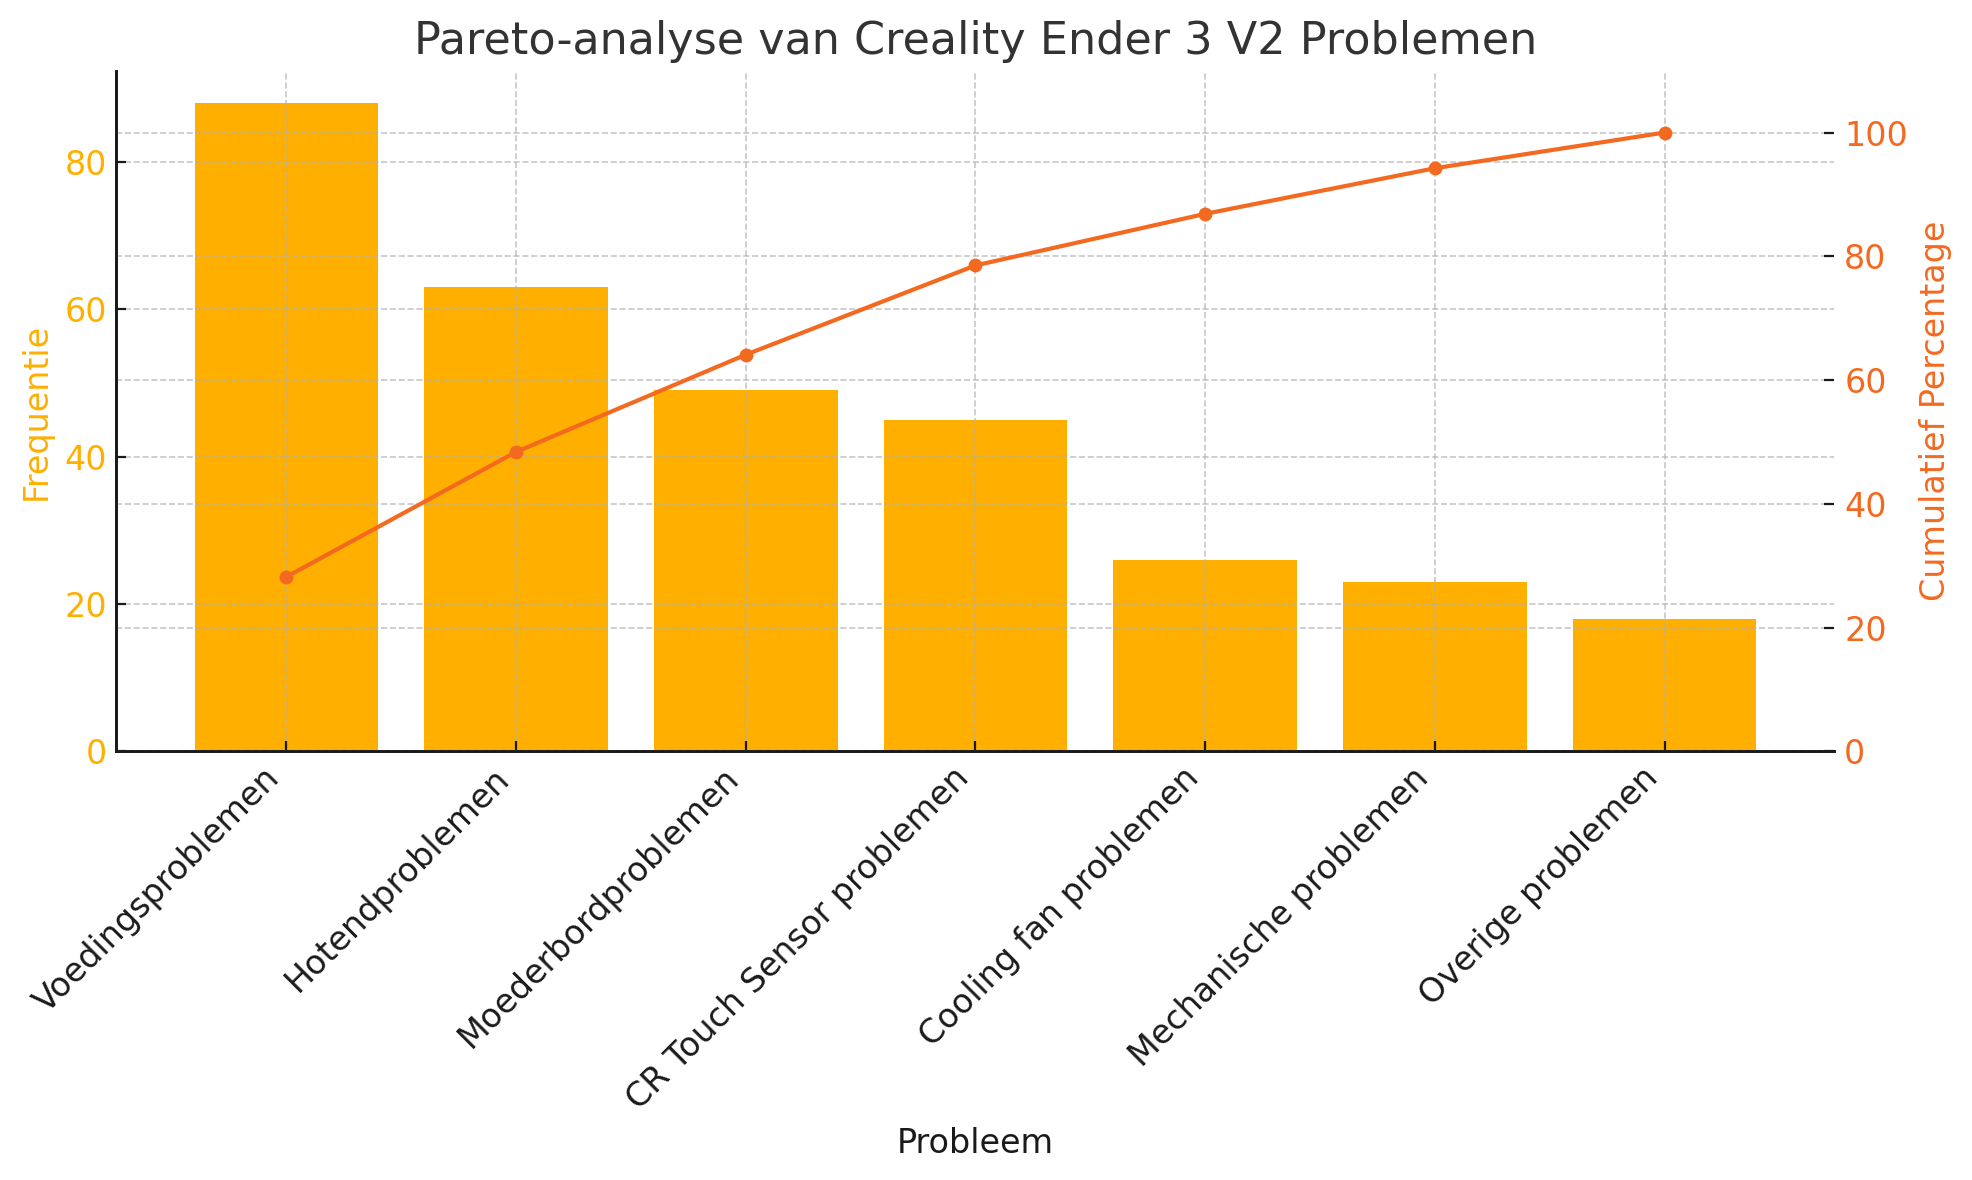
\includegraphics[width=\textwidth]{pareto_diagram.png} % Voeg hier de juiste afbeeldingsnaam in
    \caption{Pareto-diagram van Creality Ender 3 V2 Problemen}
    \label{fig:pareto}
\end{figure}

\subsection{Root Cause Analysis}
Na het uitvoeren van de Pareto-analyse, zijn de volgende root causes geïdentificeerd voor de meest voorkomende problemen:

\textbf{Voedingsproblemen}
De voeding blijkt het meest voorkomende probleem te zijn. Tijdens het onderzoek kwam naar boven dat oververhitting en stroompieken vaak de hoofdoorzaken zijn. Talrijke gebruikers hebben gemeld dat de voeding oververhit raakt als gevolg van onvoldoende koeling, een probleem dat te wijten is aan een ontwerpfout waarbij de ventilatieopeningen niet op de juiste plaatsen zijn geplaatst. De voeding bevindt zich aan de onderkant van de printer aan de achterzijde, waardoor deze niet adequaat zijn warmte kan afvoeren. Op verschillende fora's zijn meerdere oplossingen gevonden om het probleem te tackelen, zoals het toevoegen van zelf geprinte ventilatieroosters, het verhogen van de "voetjes" van de printer voor een betere luchtstroom eronder, of het verplaatsen van de voeding naar naast de printer in plaats van eronder. Door deze aanpassingen kan de voeding beter worden gekoeld en wordt de kans op oververhitting aanzienlijk verkleind.

\textbf{Moederbordproblemen}
Moederboard problemen zijn de tweede meest voorkomende categorie. Deze problemen zijn vaak te wijten aan firmware-updates die niet goed zijn uitgevoerd of incompatibiliteit met bepaalde upgrades. De oplossing bestaat vaak uit het zorgvuldig herflashen van de firmware en het controleren van compatibiliteit bij het installeren van nieuwe componenten. Ook komt op fora's vaak voor dat er geklaagd word over een lawaaiige stepper drivers op het moederboard. Al deze problemen kunnen worden opgelost met een nieuwe versie van het moederboard. Al gouw na de klachten zijn ze met een nieuwe versie gekomen van het moederboard, de 4.2.7 versie. Deze versie heeft een aantal verbeteringen ten opzichte van de vorige versies, zoals een betere koeling en een stillere werking van de stepper drivers.

\textbf{Hotendproblemen}
Hotendproblemen, zoals verstoppingen en temperatuurfouten, zijn eveneens veel gemeld. Deze problemen zijn vaak te wijten aan slecht onderhoud en het gebruik van inferieure filamenten. Regelmatig onderhoud en het gebruik van kwalitatief hoogwaardige filamenten kunnen deze problemen helpen voorkomen. Ook komt het vaak voor dat de printer in een stoffige omgeving staat zoals een slaapkamer waardoor er veel stof in de ventilator komt waardoor deze de hotend niet goed meer kan koelen. Ook word hierbij het stof de hotend ingeblazen waardoor deze verstopt kan raken. Het is daarom belangrijk om de printer in een schone omgeving te plaatsen en regelmatig te onderhouden. Binnen fora's zijn er ook veel oplossingen te vinden voor deze problemen, zoals het vervangen van de hotend of het installeren van een betere koelventilator. Echter is de makkelijkste upgrade die hiervoor word gedaan een mooie case of behuizing waar de printer in kan staan.

\newpage
%Bibliography
\bibliography{bib.bib}

% \newpage
% % Bijlage's 
% \appendix 

%   \section{Datasheet RE25 118745}
%     \label{app:datasheet motor}
%     \begin{figure}[htbp]
%       \centering % trim=left bottom right top
%       \includegraphics[page=1, clip, trim=0cm 0cm 0cm 0cm, scale = 0.65]{datasheet_RE25118745.pdf}
%       % \caption{datasheet RE25 118745}
%     \end{figure}
%     \cite{Maxon}


\end{document}